%%
%% Author: jarvis
%% 23/8/18
%%Preamble
\documentclass[16pt]{article}
\title{ICT Tools Lab 1: Introduction to \LaTeX}
\author{Gahan Saraiya}
\date{}

% Packages
\usepackage{array}
\usepackage{a4wide}
\usepackage{graphicx}
%\usepackage{bibentry, bibref}
\usepackage[acronym]{glossaries}
\graphicspath{ {figures/} }
\newglossaryentry{computer}
%\bibliography{referece}
{
	name=computer,
	description={is a programmable machine that receives input,
		stores and manipulates data, and provides
		output in a useful format}
}
\newacronym{lvm}{LVM}{Logical Volume Manager}
\makeglossaries

% Document
\begin{document}
\maketitle
\tableofcontents
\listoffigures

\newpage
% Abstract
\begin{abstract}
	This is basic introduction to \LaTeX in the Lab of ICT tools
\end{abstract}


\section{Introduction}
\label{intro}
\subsection{The Era of arc reactor}
\label{arc_reactor}
\hspace{20pt}
dummy content is here listed out \cite{ultron}
\begin{figure}[h]
	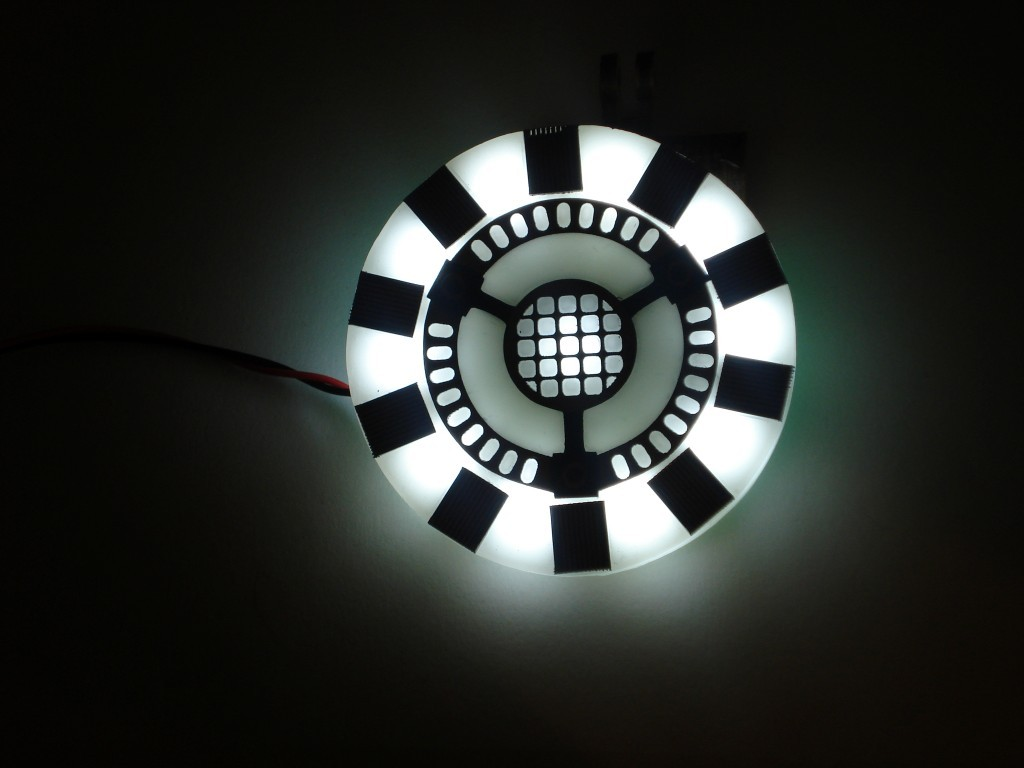
\includegraphics[scale=0.2]{arc_reactor.jpg}
\end{figure}
\\
\section{Mark 1}
\label{mk1}
\paragraph{}
Key\cite{arcReactor} to survive is the miniature version of \ref{arc_reactor} will evolve to Mark 2- \ref{mk2}.
\newline
\textbf{The key tech:}
\begin{enumerate}
	\item miniature arc reactor
	\begin{itemize}
		\item energy source
		\item A weapon?
	\end{itemize}
\end{enumerate}

\section{Mark 2}
\label{mk2}
	An achievement of stark industries private server. A truly first flying prototype.
	\begin{table}[h]
		\begin{center}
			\begin{tabular}{ |l|l|l| }
				\hline
				\textbf{ID}		&	Name & Age \\
				\hline
				1 & ABC & 35 \\
				\hline
			\end{tabular}
			\caption{table}
			\label{label1}
		\end{center}
	\end{table}

\section{Playing with equation}
	\begin{equation}
		E = mc^2
	\end{equation}
	
	\begin{equation}
		Speedup_{enhanced} = \frac{1}{(1-Fraction_{enhanced}) + (\frac{Fraction_{enhanced}}{Speedup_{enhanced}})}
	\end{equation}
	
	\begin{equation}
	y_n = y_{n-1} + \beta^2
	\end{equation}

	\begin{equation}
	\sum_{i=0}^n i^2
	\end{equation}

	\begin{equation}
	\int_{x=0}^{\pi} f(x) dx
	\end{equation}

		This is my\_table.
		\\ I \& my friend are here.\cite{7894533}

\section{References}
	\bibliographystyle{plain}
	\bibliography{reference}

\end{document}